\section{Lektion 15-02-2018}
\subsubsection{GraphicTFT display driver}

Driver for "ITDB02 320 x 240 TFT display module, Version 2" mounted at "ITDB02 Arduino Mega2560 Shield".\\

\noindent Display controller = ILI 9341.\\

\begin{tabular}{ll}
	\textbf{Connections}\\
	\hline
	\rule{0pt}{5mm}  
	DB15-DB8:   & PORT A\\ 
	\rule{0pt}{5mm}
	DB7-DB0:    & PORT C\\ 
	\rule{0pt}{5mm}
	RESETx:     & PORT G, bit 0\\ 
	\rule{0pt}{5mm}
	CSx:        & PORT G, bit 1\\ 
	\rule{0pt}{5mm}
	WRx:        & PORT G, bit 2\\ 
	\rule{0pt}{5mm}
	RS (=D/Cx): & PORT D, bit 7\\ 
\end{tabular} 

\begin{minted}{c}
// Data port definitions:
#define DATA_PORT_HIGH PORTA
#define DATA_PORT_LOW  PORTC

// Control port definitions:
#define WR_PORT PORTG
#define WR_BIT 2
#define DC_PORT PORTD
#define DC_BIT  7  // SHIELD RS
#define CS_PORT PORTG
#define CS_BIT  1
#define RST_PORT PORTG
#define RST_BIT 0
\end{minted}
Start by implementing the basic, time-critical functions.

\begin{figure} [H]
	\centering
	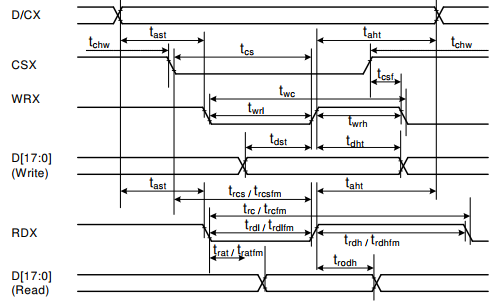
\includegraphics[width=0.8\linewidth]{graphics/LAB3a.png}
	\caption{Timing Characteristics (8080-Ⅰ system).}
	\label{fig:11}
\end{figure}

\noindent\mintinline{c}{PORTD &= ~(1 << n);} will set PIN n low.\\

\noindent\mintinline{c}{PORTD |= (1 << n);} will set PIN n high.

\begin{minted}{c}
void WriteCommand(unsigned int command)
{
DATA_PORT_LOW = command;
DC_PORT &= ~(1<<DC_BIT);       // DCX LOW = COMMAND MODE
CS_PORT &= ~(1<<CS_BIT);       // CSX LOW
WR_PORT &= ~(1<<WR_BIT);       // WRX LOW
_NOP();			// DELAY = twrl 15ns
WR_PORT |= (1<<WR_BIT);	// WRX HIGH
_NOP();			// DELAY = tcf 10ns
}
\end{minted}

\begin{minted}{c}
void WriteData(unsigned int data)
{
DATA_PORT_HIGH = (data >> 8);	// MSB
DATA_PORT_LOW  = data;	       // LSB
DC_PORT |= (1<<DC_BIT);	      // DCX HIGH = DATA MODE
CS_PORT &= ~(1<<CS_BIT);	     // CSX LOW
WR_PORT &= ~(1<<WR_BIT);	     // WRX LOW
_NOP();			      // DELAY = twrl 15ns
WR_PORT |= (1<<WR_PORT);	     // WRX HIGH
_NOP();			      // DELAY = twcf 10ns
}
\end{minted}